\documentclass[tikz,border=3.14pt]{standalone}
\makeatletter%
\tikzset{%
  rel/.code={%
    \pgfsetlinetofirstplotpoint%
    \edef\rel@curr@x{\the\tikz@lastx}%
    \edef\rel@curr@y{\the\tikz@lasty}%
    \let\rel@plot\tikz@@@plot
    \def\tikz@@@plot{%
      \let\rel@streampoint\pgfplotstreampoint
      \def\pgfplotstreampoint####1{%
        \pgf@process{####1}%
        \advance\pgf@x by \rel@curr@x\relax
        \advance\pgf@y by \rel@curr@y\relax
        \edef\rel@point{\noexpand\rel@streampoint{\noexpand\pgfqpoint{\the\pgf@x}{\the\pgf@y}}}%
        \rel@point
      }%
      \rel@plot
    }
  }
}
\makeatother
\begin{document}
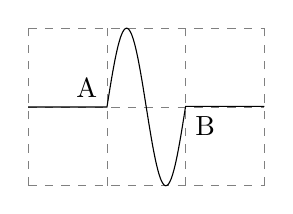
\begin{tikzpicture}
\draw[help lines, dashed] (0,0) grid (3,2);
\draw 
    (0,1) -- (1,1) node[above left] {A}
    plot[rel, domain=0:1, samples=100, smooth] (\x, {sin(6.3*\x r)}) node[below right] {B}
    -- ++(1, 0)
;
\end{tikzpicture}
\end{document}
